\paragraph{}{
	Le second circuit éléectronique composant le processeur est
	le contrôleur de saut. Son rôle est de mettre à jour \textit{PC}
	à jour en fonction du résultat de l'opération que vient d'effectuer
	l'UAL pour le cycle suivant.
	Le saut est déterminé en fonction des indicateurs que le circuits
	à en entrées, c'est-à-dire \textit{SF} et \textit{ZF}.
}

\begin{figure}[!ht]
	\centering
	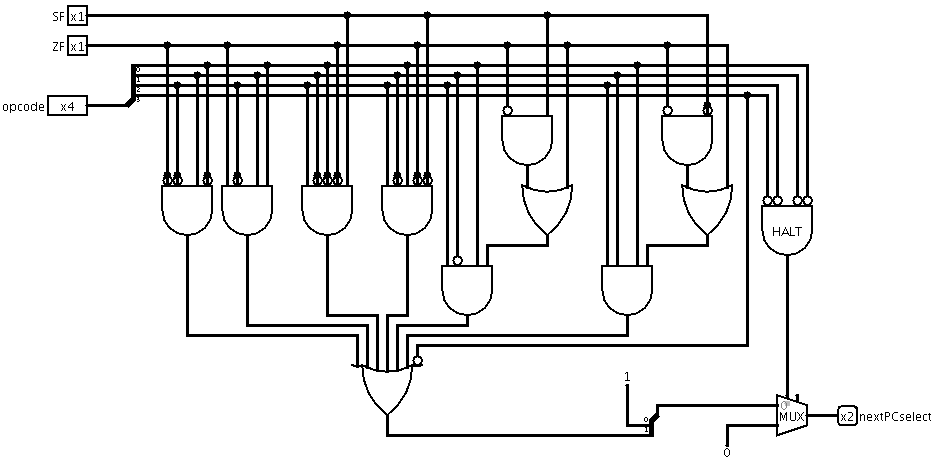
\includegraphics[scale=0.4,origin=c]{circuits/control_saut.png}
	\label{control_saut_circ}
	\caption{Sch\'{e}ma \'{e}lectronique du contr\^{o}leur de sauts}
\end{figure}

\paragraph{}{
	Le schéma électronique du contrôleur de saut est à la figure
	\ref{control_saut_circ}. 
}